\documentclass[tikz,border=3pt]{standalone}
\usepackage[T1]{fontenc}
\usepackage{mathptmx}
\usepackage{amsmath}
\usetikzlibrary{arrows.meta,positioning,shapes.geometric,fit,backgrounds,calc,decorations.pathreplacing}

\definecolor{nav}{RGB}{31,78,156}
\definecolor{navl}{RGB}{232,238,248}
\definecolor{red}{RGB}{178,34,34}
\definecolor{redl}{RGB}{250,233,233}
\definecolor{grn}{RGB}{46,125,50}
\definecolor{grnl}{RGB}{231,243,232}
\definecolor{gry}{RGB}{90,90,90}
\definecolor{gryl}{RGB}{240,240,240}
\definecolor{lane}{RGB}{248,248,248}

\tikzset{
  every node/.style={font=\fontsize{6.8}{7.8}\selectfont, inner sep=1.5pt},
  blk/.style={draw=black!85, line width=0.5pt, rounded corners=1.5pt, fill=white},
  ttl/.style={font=\fontsize{7.4}{8}\selectfont\bfseries, align=center},
  small/.style={font=\fontsize{5.8}{6.6}\selectfont},
  flow/.style={-{Stealth[length=3.4pt,width=2.8pt]}, line width=0.55pt},
  dflow/.style={-{Stealth[length=3pt,width=2.4pt]}, line width=0.5pt, densely dashed, gry},
  nb/.style={circle, fill=black, text=white, font=\fontsize{5.8}{6}\selectfont\bfseries, inner sep=0pt, minimum size=9.5pt},
  nr/.style={circle, fill=red, text=white, font=\fontsize{5.8}{6}\selectfont\bfseries, inner sep=0pt, minimum size=9.5pt},
}

\newcommand{\server}[2]{% lower-left corner
  \foreach \i in {0,1,2}{
    \draw[line width=0.4pt, fill=white] (#1,#2+\i*0.2) rectangle ++(0.75,0.17);
    \fill[grn] (#1+0.1,#2+\i*0.2+0.085) circle (0.022);
    \draw[line width=0.3pt] (#1+0.28,#2+\i*0.2+0.085) -- ++(0.37,0);}}
\newcommand{\person}[3]{% x,y of head centre, colour
  \fill[#3] (#1,#2) circle (0.085);
  \draw[#3, line width=1.1pt] (#1-0.15,#2-0.2) arc (180:0:0.15);}

\begin{document}
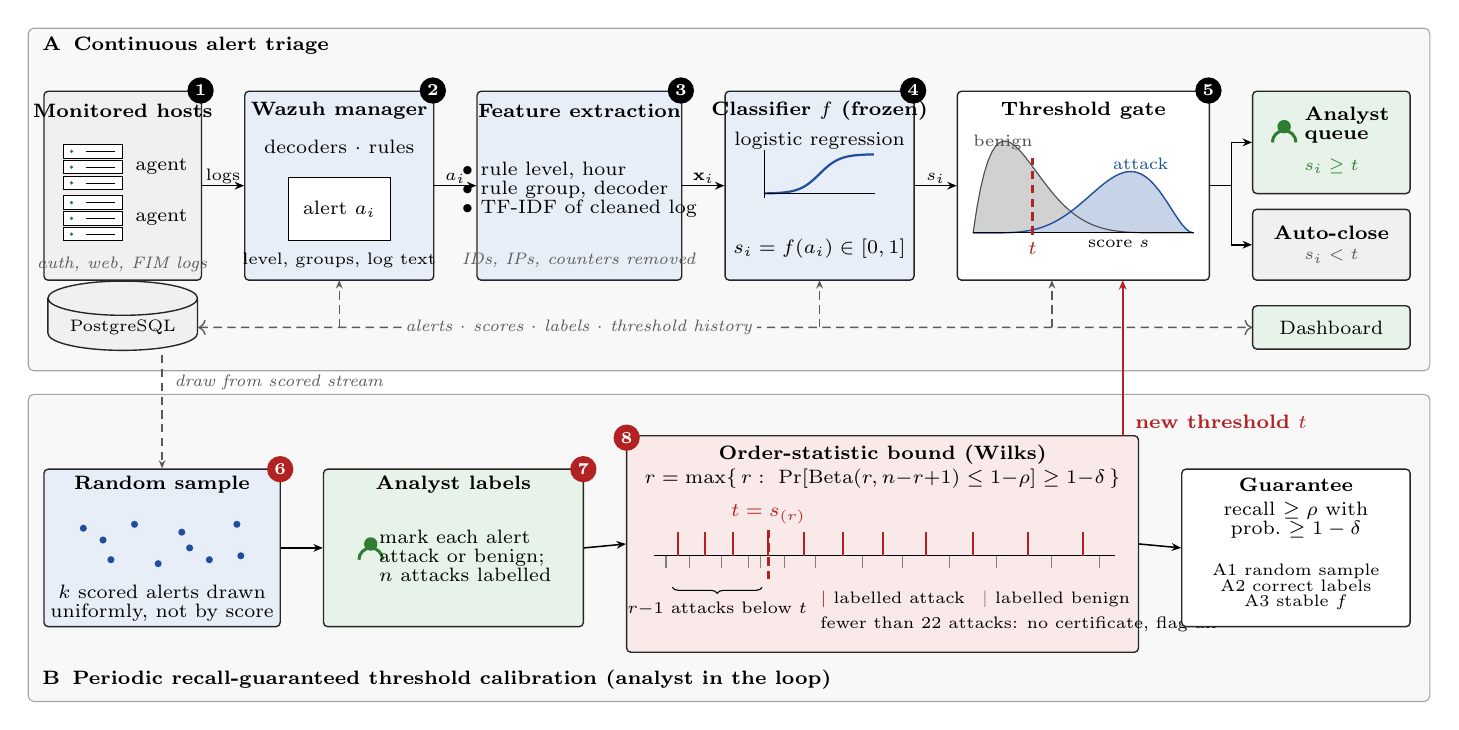
\begin{tikzpicture}[x=1cm,y=1cm]

% ---------------- lanes
\begin{scope}[on background layer]
  \draw[draw=black!35, fill=lane, rounded corners=2pt, line width=0.4pt] (0,4.2) rectangle (17.8,8.55);
  \draw[draw=black!35, fill=lane, rounded corners=2pt, line width=0.4pt] (0,0) rectangle (17.8,3.9);
\end{scope}
\node[ttl, anchor=north west] at (0.12,8.5) {A\enspace Continuous alert triage};
\node[ttl, anchor=south west] at (0.12,0.1) {B\enspace Periodic recall-guaranteed threshold calibration (analyst in the loop)};

% ================= LANE A  (row centre y = 6.55, box height 2.4)
% hosts
\node[blk, fill=gryl, minimum width=2.0cm, minimum height=2.4cm] (hosts) at (1.2,6.55) {};
\node[ttl] at (1.2,7.5) {Monitored hosts};
\server{0.45}{6.5} \node[anchor=west] at (1.3,6.8) {agent};
\server{0.45}{5.85} \node[anchor=west] at (1.3,6.15) {agent};
\node[small, gry] at (1.2,5.55) {\textit{auth, web, FIM logs}};
% manager
\node[blk, fill=navl, minimum width=2.4cm, minimum height=2.4cm] (mgr) at (3.95,6.55) {};
\node[ttl] at (3.95,7.5) {Wazuh manager};
\node at (3.95,7.05) {decoders $\cdot$ rules};
\draw[line width=0.4pt, fill=white] (3.3,5.85) rectangle (4.6,6.65);
\node at (3.95,6.25) {alert $a_i$};
\node[small] at (3.95,5.6) {level, groups, log text};
% features
\node[blk, fill=navl, minimum width=2.6cm, minimum height=2.4cm] (feat) at (7.0,6.55) {};
\node[ttl] at (7.0,7.5) {Feature extraction};
\node[align=left] at (7.0,6.5) {$\bullet$ rule level, hour\\[-1pt]$\bullet$ rule group, decoder\\[-1pt]$\bullet$ TF-IDF of cleaned log};
\node[small, gry] at (7.0,5.6) {\textit{IDs, IPs, counters removed}};
% classifier
\node[blk, fill=navl, minimum width=2.4cm, minimum height=2.4cm] (clf) at (10.05,6.55) {};
\node[ttl] at (10.05,7.5) {Classifier $f$ (frozen)};
\draw[nav, line width=0.8pt, domain=-0.6:0.6, samples=30] plot ({10.05+\x*1.15},{6.45+0.5/(1+exp(-9*\x))});
\draw[line width=0.35pt] (9.35,6.45) -- (10.75,6.45); \draw[line width=0.35pt] (9.35,6.4) -- (9.35,7.0);
\node at (10.05,7.12) {logistic regression};
\node at (10.05,5.75) {$s_i=f(a_i)\in[0,1]$};
% gate
\node[blk, minimum width=3.2cm, minimum height=2.4cm] (gate) at (13.4,6.55) {};
\node[ttl] at (13.4,7.5) {Threshold gate};
\begin{scope}[shift={(12.0,5.95)}, xscale=2.8, yscale=1.0]
  \fill[black!18] plot[domain=0:1,samples=60] (\x,{20.6*\x*(1-\x)^6}) -- (1,0) -- (0,0) -- cycle;
  \fill[nav!25]   plot[domain=0:1,samples=60] (\x,{0.78*65.9*\x^5*(1-\x)^2}) -- (1,0) -- (0,0) -- cycle;
  \draw[black!70, line width=0.4pt] plot[domain=0:1,samples=60] (\x,{20.6*\x*(1-\x)^6});
  \draw[nav, line width=0.5pt]     plot[domain=0:1,samples=60] (\x,{0.78*65.9*\x^5*(1-\x)^2});
  \draw[line width=0.4pt] (0,0) -- (1,0);
  \draw[red, line width=0.9pt, densely dashed] (0.27,-0.02) -- (0.27,0.95);
  \node[red, anchor=north, font=\fontsize{7.4}{8}\selectfont] at (0.27,-0.06) {$t$};
  \node[anchor=south west, small, black!70] at (-0.02,1.0) {benign};
  \node[small, nav] at (0.76,0.88) {attack};
  \node[small, anchor=north] at (0.66,-0.04) {score $s$};
\end{scope}
% outputs
\node[blk, fill=grnl, minimum width=2.0cm, minimum height=1.3cm] (queue) at (16.55,7.1) {};
\person{15.95}{7.3}{grn}
\node[anchor=west, align=left] at (16.15,7.32) {\textbf{Analyst}\\[-1pt]\textbf{queue}};
\node[grn, small] at (16.55,6.8) {$s_i\geq t$};
\node[blk, fill=gryl, minimum width=2.0cm, minimum height=0.9cm] (close) at (16.55,5.8) {};
\node at (16.55,5.95) {\textbf{Auto-close}};
\node[gry, small] at (16.55,5.65) {$s_i<t$};

\draw[flow] (hosts.east) -- (mgr.west);
\draw[flow] (mgr.east) -- (feat.west);
\draw[flow] (feat.east) -- (clf.west);
\draw[flow] (clf.east) -- (gate.west);
\draw (gate.east) -- (15.28,6.55);
\draw[flow] (15.28,6.55) |- (queue.west);
\draw[flow] (15.28,6.55) |- (close.west);
\node[small, anchor=south, inner sep=0.5pt] at ($(hosts.east)!0.5!(mgr.west)$) {logs};
\node[small, anchor=south, inner sep=0.5pt] at ($(mgr.east)!0.5!(feat.west)$) {$a_i$};
\node[small, anchor=south, inner sep=0.5pt] at ($(feat.east)!0.5!(clf.west)$) {$\mathbf{x}_i$};
\node[small, anchor=south, inner sep=0.5pt] at ($(clf.east)!0.5!(gate.west)$) {$s_i$};
\foreach \x/\n in {hosts/1,mgr/2,feat/3,clf/4,gate/5}{ \node[nb] at ($(\x.north east)+(-0.02,0)$) {\n}; }

% data store + bus
\node[cylinder, shape border rotate=90, aspect=0.3, draw=black!85, line width=0.5pt, fill=gryl, minimum height=0.75cm, minimum width=1.9cm, font=\fontsize{6.4}{7}\selectfont] (db) at (1.2,4.75) {PostgreSQL};
\node[blk, fill=grnl, minimum width=2.0cm, minimum height=0.55cm] (dash) at (16.55,4.75) {Dashboard};
\draw[dflow, <->] (db.east) -- (dash.west);
\foreach \x in {3.95,10.05,13.0}{ \draw[dflow] (\x,4.75) -- (\x,5.35); }
\node[small, gry, fill=lane, inner sep=1.2pt] at (7.0,4.75) {\textit{alerts $\cdot$ scores $\cdot$ labels $\cdot$ threshold history}};

% ================= LANE B  (row centre y = 1.95)
\node[blk, fill=navl, minimum width=3.0cm, minimum height=2.0cm] (samp) at (1.7,1.95) {};
\node[ttl] at (1.7,2.75) {Random sample};
\foreach \p in {(0.7,2.2),(1.05,1.8),(1.35,2.25),(1.65,1.75),(1.95,2.15),(2.3,1.8),(2.65,2.25),(0.95,2.05),(2.05,1.95),(2.7,1.85)} { \fill[nav] \p circle (0.045); }
\node[align=center] at (1.7,1.25) {$k$ scored alerts drawn\\[-1pt]uniformly, not by score};
\node[nr] at (3.2,2.95) {6};

\node[blk, fill=grnl, minimum width=3.3cm, minimum height=2.0cm] (lab) at (5.4,1.95) {};
\node[ttl] at (5.4,2.75) {Analyst labels};
\person{4.35}{2.0}{grn}
\node[align=left] at (5.55,1.85) {mark each alert\\[-1pt]attack or benign;\\[-1pt]$n$ attacks labelled};
\node[nr] at (7.05,2.95) {7};

\node[blk, fill=redl, minimum width=6.5cm, minimum height=2.75cm] (bound) at (10.85,2.0) {};
\node[ttl] at (10.85,3.14) {Order-statistic bound (Wilks)};
\node at (10.85,2.83) {$r=\max\{\,r:\ \Pr[\mathrm{Beta}(r,n{-}r{+}1)\le 1{-}\rho]\ge 1{-}\delta\,\}$};
\draw[line width=0.5pt] (7.95,1.85) -- (13.8,1.85);
\foreach \x in {8.25,8.6,8.95,9.4,9.85,10.35,10.85,11.4,12.0,12.7,13.4}{ \draw[red, line width=0.75pt] (\x,1.85) -- ++(0,0.3); }
\foreach \x in {8.1,8.4,8.8,9.15,9.3,9.6,10.0,10.6,11.1,11.7,12.3,13.0,13.6}{ \draw[black!50, line width=0.4pt] (\x,1.85) -- ++(0,-0.16); }
\draw[line width=0.85pt, red, densely dashed] (9.4,1.55) -- (9.4,2.22);
\node[red, anchor=south] at (9.4,2.2) {$t=s_{(r)}$};
\draw[decorate, decoration={brace,amplitude=2.2pt,mirror}, line width=0.4pt] (8.18,1.45) -- (9.32,1.45);
\node[small] at (8.75,1.17) {$r{-}1$ attacks below $t$};
\node[small, anchor=west] at (10.0,1.3) {\textcolor{red}{$|$} labelled attack \enspace \textcolor{black!50}{$|$} labelled benign};
\node[small, anchor=west] at (10.0,0.98) {fewer than 22 attacks: no certificate, flag all};
\node[nr] at (7.6,3.35) {8};

\node[blk, minimum width=2.9cm, minimum height=2.0cm] (guar) at (16.1,1.95) {};
\node[ttl] at (16.1,2.75) {Guarantee};
\node[align=center] at (16.1,2.3) {recall $\ge\rho$ with\\[-1pt]prob.\ $\ge 1-\delta$};
\node[small, align=center] at (16.1,1.45) {A1 random sample\\[-1pt]A2 correct labels\\[-1pt]A3 stable $f$};

\draw[flow] (samp.east) -- (lab.west);
\draw[flow] (lab.east) -- (bound.west);
\draw[flow] (bound.east) -- (guar.west);
% stream into sampler
\draw[dflow] (1.7,4.4) -- (samp.north);
\node[small, gry, anchor=west] at (1.8,4.05) {\textit{draw from scored stream}};
% feedback
\draw[flow, red, line width=0.85pt] (13.9,3.375) -- (13.9,5.35);
\node[red, anchor=west, font=\fontsize{6.8}{7.6}\selectfont\bfseries] at (14.0,3.55) {new threshold $t$};

\end{tikzpicture}
\end{document}
